%-------------------------------------------------------------------------------
%   PACKAGES EN CONFIGURATIE
%-------------------------------------------------------------------------------

\documentclass{uva-inf-presentation}
\usepackage[british]{babel}
\usepackage{listings}
\usepackage{tikz}
\usepackage{environ}

\usepackage{caption}
\DeclareCaptionFont{white}{\color{white}}
\DeclareCaptionFormat{listing}{\colorbox{gray}{{#3}}}
\captionsetup[lstlisting]{format=listing,labelfont=white,textfont=white}

\uselanguage{Dutch}
\languagepath{Dutch}

%-------------------------------------------------------------------------------
%   TITELPAGINA EN INHOUDSOPGAVE
%-------------------------------------------------------------------------------

% Een korte titel voor de footer, een langere titel voor de titelpagina
\title[Breaking Traditional Ciphers]{\small{Information and Communication}\\\textbf{Codebreaking for Traditional Cipher Systems}}

% Vul beide namen hier in
\author{Abe Wiersma}
\institute[UvA]{
\includegraphics[width=6cm]{logoUvA_nl}}
\date{\today}

\begin{document}

\begin{frame}
% De eerste slide is de titelpagina
\titlepage
\end{frame}

\begin{frame}
% Geeft een inhoudsopgave voor de presentatie
\frametitle{Table of Contents}
\tableofcontents
\end{frame}

%-------------------------------------------------------------------------------
%   PRESENTATIE SLIDES
%-------------------------------------------------------------------------------

% Secties zijn er om structuur in je presentatie aan te brengen
% en worden direct in de inhoudsopgave opgenomen
\section{Introduction in Ciphers}
%################################################
% Maak een subsection voor een serie slides met een gedeeld thema

%------------------------------------------------
\subsection{Communication}
%------------------------------------------------

\begin{frame}
\frametitle{Communication}

%% Document
\begin{center}
\resizebox{\textwidth}{!}{%
    \begin{tikzpicture}[]
        \tikzstyle{every node}=[transform shape];

        % Alice
        \node (label) at (0,0) {\includegraphics[height=7cm]{canal_alice_dep.pdf}};
        \node (label) at (0,-4) {\Huge\bf Alice};

        % Bob
        \node (label) at (30,0) {\includegraphics[height=7cm]{canal_bob_dep.pdf}};
        \node (label) at (30,-4) {\Huge\bf Bob};

        % Eve
        \node (label) at (15,-6) {\includegraphics[height=7cm]{canal_eve_dep.pdf}};
        \node (label) at (15,-10) {\Huge\bf Eve};
        \draw[->, line width=1mm] (12,-7) -- ++(-3,0) -- node[left] {\Huge\bf Listen} ++(0,+5.5);
        \draw[->, line width=1mm] (18,-7) -- ++(+3,0) --  node[right] {\Huge\bf Modify} ++(0,+5.5);

        % Canal
        \draw[line width=1mm] (4,-1) ellipse (0.7 and 1);
        \draw[line width=1mm] (25,-2) arc (-90:90:1);

        \draw[line width=1mm] (4,0) -- ++(21,0);
        \draw[line width=1mm] (4,-2) -- ++(21,0);
        \node (label) at (14.5, 0.5) {\Huge\bf Unsecured canal of communication};
    \end{tikzpicture}
}%
\end{center}
\end{frame}

%------------------------------------------------
\subsection{Ciphers}
%------------------------------------------------

\begin{frame}
\frametitle{Ciphers}

\textbf{Cipher:}\\
Algorithm that maps Input to Output(enciphered text).\\
Maps back from the enciphered text to the Input. With or without key.

\end{frame}

\begin{frame}
\frametitle{'Safe' communication}

%% Document
\begin{center}
\resizebox{\textwidth}{!}{%
    \begin{tikzpicture}[]
        \tikzstyle{every node}=[transform shape];

        % Alice
        \node (label) at (0,0) {\includegraphics[height=7cm]{canal_alice_dep.pdf}};
        \node (label) at (0,-4) {\Huge\bf Alice};

        \draw[->, line width=1mm] (2,-1) -- (3,-1);
        \node[rectangle, draw, font=\fontsize{35}{80}\selectfont, minimum height=2cm]  at (5,-1) {Encode};
        \draw[->, line width=1mm] (7,-1) -- (8,-1);

        % Canal
        \draw[line width=1mm] (8,-1) ellipse (0.7 and 1);
        \draw[line width=1mm] (21,-2) arc (-90:90:1);
        \draw[line width=1mm] (8,0) -- ++(13,0);
        \draw[line width=1mm] (8,-2) -- ++(13,0);
        \node (label) at (14.5, 0.5) {\Huge\bf Canal of communication};
        % \Canal

        % Bob
        \node (label) at (30,0) {\includegraphics[height=7cm]{canal_bob_dep.pdf}};
        \node (label) at (30,-4) {\Huge\bf Bob};

        \draw[->, line width=1mm] (21.5,-1) -- (22.5,-1);
        \node[rectangle, draw, font=\fontsize{35}{80}\selectfont, minimum height=2cm]  at (24.5,-1) {Decode};
        \draw[->, line width=1mm] (26.5,-1) -> (28,-1);

        % Eve
        \node (label) at (15,-6) {\includegraphics[height=7cm]{canal_eve_dep.pdf}};
        \node (label) at (15,-10) {\Huge\bf Eve};
        \draw[->, line width=1mm] (12,-7.5) -- ++(-2,0) -- node[left] {\Huge\bf Listen} ++(0,+5.5);
        \draw[->, line width=1mm] (18,-7.5) -- ++(+2,0) --  node[right] {\Huge\bf Modify} ++(0,+5.5);

    \end{tikzpicture}
}%
\end{center}
\end{frame}

%------------------------------------------------
\subsection{Traditional Ciphers}
%------------------------------------------------

\begin{frame}
\frametitle{Traditional Ciphers}
\textbf{History:}
\begin{itemize}
    \item Origin lies in ancient Egypt $\sim4000$ years ago. %mostly army/government
    \item Ends after second world war with the emergence of the computers.
\end{itemize}
\textbf{Uses}:
\begin{itemize}
    \item War movement.
    \item Government Secrets.
\end{itemize}
\end{frame}

\section{Breaking Traditional Ciphers}

\begin{frame}
\frametitle{Types: Traditional Ciphers}
\begin{itemize}
    \item Substitution Cipher
    \item Permutation Cipher
    \item Substitution and Permutation Cipher.
    \item Running key Cipher
    \item An Enigma-style periodic poly-alphabetic Cipher
\end{itemize}
\end{frame}

\subsection{Substitution Cipher}
\frame{\tableofcontents[currentsubsection]}

\begin{frame}
\frametitle{Substitution Cipher:\\ Example}
A Caesar Cipher is a Substitution Cipher that shifts a regular alphabet.
Here a Caesar Cipher with a right shift of 3:\\
\begin{table}
    \begin{tabular}{lc}
        Plain:  & ABCDEFGHIJKLMNOPQRSTUVWXYZ\\
        Cipher: & XYZABCDEFGHIJKLMNOPQRSTUVW
    \end{tabular}
\end{table}

Decoding a Caesar Cipher text with our Caesar cipher.\\
\textbf{Ciphertext:}\\
\hspace{4ex}QEB NRFZH YOLTK CLU GRJMP LSBO QEB IXWV ALD
\textbf{Decoded Plaintext:}\\
\hspace{4ex}THE QUICK BROWN FOX JUMPS OVER THE LAZY DOG
\end{frame}

\begin{frame}
\frametitle{Substitution Cipher:\\ Problem}
\vspace{-20pt}
\lstinputlisting[
    backgroundcolor=\color{lightgray},
    breakindent=0.5pt,
    breaklines,
    basicstyle=\tiny,
    caption=Substitution Cipher provided by Mathias,
]{ciphers/substitution_cipher.txt}

\end{frame}

\begin{frame}
\frametitle{Substitution Cipher:\\ Solution}
Finding the solution is a process of small increments.

\begin{minipage}{0.55\linewidth}
Analysis of the Cipher text gives us the number of different characters:
35\\
And also gives us the frequencies of the characters $\rightarrow$
\end{minipage}%
\begin{minipage}{0.45\linewidth}
\centering
{\fontsize{3.5pt}{4.5pt}\selectfont
\begin{tabular}{ll}\toprule
Character & Frequency in \%     \\
\midrule
p         & 16.86 \\
r         & 10.83 \\
1         & 6.723 \\
;         & 6.296 \\
l         & 6.083 \\
h         & 5.869 \\
:         & 5.763 \\
8         & 5.336 \\
z         & 5.336 \\
9         & 4.268 \\
w         & 3.361 \\
y         & 3.201 \\
i         & 2.401 \\
e         & 2.401 \\
n         & 2.187 \\
s         & 1.867 \\
          & 1.814 \\
f         & 1.440 \\
o         & 1.387 \\
-         & 1.334 \\
7         & 1.334 \\
c         & 1.173 \\
v         & 0.907 \\
d         & 0.640 \\
t         & 0.266 \\
x         & 0.213 \\
q         & 0.213 \\
a         & 0.106 \\
.         & 0.053 \\
,         & 0.053 \\
k         & 0.053 \\
b         & 0.053 \\
u         & 0.053 \\
g         & 0.053 \\
m         & 0.053 \\ \bottomrule
\end{tabular}}
\end{minipage}
\end{frame}

\begin{frame}
\frametitle{Substitution Cipher:\\ Solution}
A space is the most common character in the English language,
which implies p decoded is ' `\\

We can also apply that the most common letter in the English language is the
letter e, which implies that r decoded is 'e`
\end{frame}

\begin{frame}[containsverbatim]
\frametitle{Substitution Cipher:\\ Solution}
\vspace{-20pt}
\begin{lstlisting}[
    backgroundcolor=\color{lightgray},
    breakindent=0.5pt,
    breaklines,
    basicstyle=\tiny,
    caption=Substitution Cipher provided by Mathias,
]
eVeZF19;:- :8O -8eH 8: L1 19e -LYY8 D 19eZe ;H L ZL;YOLF H eeW ;: 19e H1;ZZ;:- 8E 19e S;:WC :81 YeHH 19L: ;: 19e S8VeSe:1 8E 19e 78W;eH 8E Se:D 19e H8N;LY L:W  8Y;1;NLY  LHH;8:H 9LVe LNMI;ZeW HIN9 ;:1e:H;1FC L:W 7ee: H8 O;WeYF W;EEIHeWC 19L1 19e;Z ;:eV;1L7Ye ZeHIY1H LZe LYS8H1 ;SSeW;L1eYF  Z8WINeWD 19e  eZ;8W 8E HeeWA1;Se L:W 9LZVeH1 9LH 7eN8Se LH H98Z1 ;:  8Y;1;NLY LH ;1 ;H ;: L-Z;NIY1IZLY YL78IZD L H;:-Ye FeLZ 7Z;:-H ;1H L  Z8 Z;L1e EZI;1H 18 SL1IZ;1F ;: 19e S8ZLY LH ;: 19e  9FH;NLY O8ZYWD e;-91F FeLZH eYL HeW ;: Z8Se EZ8S 19e 1;Se O9e: 19e  8Y;1;NLY  LHH;8:H OeZe E;ZH1 H1;ZZeW 7F 1;7eZ;IH -ZLNN9IHC 7eE8Ze ;1H I:ZIYF N;1;Ke:H OeZe E;:LYYF HI7WIeW 7F 19e LZ1C 8Z WeN;SL1eW 7F 19e NZIeY1F 8E 8N1LV;IHD e:-YL:W I:WeZOe:1 H;X FeLZH 8E N;V;Y OLZ L:W HIEEeZ;:-C 7eE8Ze 19e LS7;1;8: L:W SLW:eHH 8E 19e Y8:-  LZY;LSe:1 OeZe eX eYYeW 7F 19e  IZ-e 8E  Z;WeC 8Z NZIH9eW 7F 19e HO8ZW 8E NZ8SOeYYB 1OeYVe FeLZH eYL HeW 7e1Oee: 19e N8:V8NL1;8: 8E 19e H1L1eHA-e:eZLY ;: ,U.GC L:W 19e eX1;:N1;8: 8E 19e Y;Ne:He 8E 19e EZe:N9 ZeV8YI1;8: 7F 19e LZS 8E :L 8Ye8:D 7I1C 8: 19;H 8NNLH;8:C ;: 8:e FeLZC LYYC ;: 19e SeL:1;Se L1 YeLH1C 9LH 7ee: LNN8S Y;H9eWD eZe 19e YeLVeHC O9;N9 I:E8YWeW ;: H Z;:- LS;WH1 19e 8VeZ19Z8O 8E 19Z8:eHC L:W 19e 1ZL:H 8Z1H 8E ZeV8YI1;8:;H1H 8VeZ 19e O8ZYWC 9LW ELYYe: ;: LI1IS:C 19e  LHH;8:H O9;N9 9LW N8:VIYHeW SL:T;:W OeZe NZIH9eW E8Z 19e 1;SeC L:W 19e 1Z;IS 9H 8E WeS8NZLNF OeZe LZZeH1eWD L 1eZZ;7Ye ZeLN1;8: 9LW He1 ;:Q eX eZ;e:Ne 8E HIEEeZ;:- 9LW W8:e ;1H O8ZTQ L:W HO;E1 LH 19e H9LWeH 8E :;-91 7eE8Ze 19e ZLFH 8E 19e LHNe:W;:- HI:C 9LW W;HL  eLZeW 19e EeZSe:1 8E ZeV8YI1;8: 7eE8Ze 19e LZ8IHeW ;:W;-:L1;8: 8E 19e I:N8ZZI 1eW  LZ1 8E SL:T;:WD 19e HLSe  LHH;8:H SLF L-L;: LZ;HeQ 19e HLSe WeYIH;8:H L-L;: H ZeLWC LH H;: H Z;:-H I  LEZeH9 ;: HINNeHH;Ve -e:eZL1;8:H 8E Se:Q 7I1 Oe T:8O 19e ZeHIY1D 19eF O;YYC Y;Te 19e OLFH 8E 19e I:Z;-91e8IHC 7e L-L;: NZIH9eWD
\end{lstlisting}
\end{frame}

\begin{frame}
\frametitle{Substitution Cipher:\\ Solution}
So this intermediate step contains a lot of 19e, and the is the most common
trigram in the English language. 19e decoded is the.
\end{frame}

\begin{frame}[containsverbatim]
\frametitle{Substitution Cipher:\\ Solution}
\vspace{-20pt}
\begin{lstlisting}[
    backgroundcolor=\color{lightgray},
    breakindent=0.5pt,
    breaklines,
    basicstyle=\tiny,
    caption=Substitution Cipher provided by Mathias,
]
evezfth;:- :8o -8eh 8: lt the -lyy8 d theze ;h l zl;yolf h eew ;: the ht;zz;:- 8e the s;:wc :8t yehh thl: ;: the s8vese:t 8e the 78w;eh 8e se:d the h8n;ly l:w  8y;t;nly  lhh;8:h hlve lnmi;zew hinh ;:te:h;tfc l:w 7ee: h8 o;weyf w;eeihewc thlt the;z ;:ev;tl7ye zehiyth lze lys8ht ;ssew;lteyf  z8winewd the  ez;8w 8e heewat;se l:w hlzveht hlh 7en8se lh hh8zt ;:  8y;t;nly lh ;t ;h ;: l-z;niytizly yl78izd l h;:-ye felz 7z;:-h ;th l  z8 z;lte ezi;th t8 sltiz;tf ;: the s8zly lh ;: the  hfh;nly o8zywd e;-htf felzh eyl hew ;: z8se ez8s the t;se ohe: the  8y;t;nly  lhh;8:h oeze e;zht ht;zzew 7f t;7ez;ih -zlnnhihc 7ee8ze ;th i:ziyf n;t;ke:h oeze e;:lyyf hi7wiew 7f the lztc 8z wen;sltew 7f the nzieytf 8e 8ntlv;ihd e:-yl:w i:wezoe:t h;x felzh 8e n;v;y olz l:w hieeez;:-c 7ee8ze the ls7;t;8: l:w slw:ehh 8e the y8:-  lzy;lse:t oeze ex eyyew 7f the  iz-e 8e  z;wec 8z nzihhew 7f the ho8zw 8e nz8soeyyb toeyve felzh eyl hew 7etoee: the n8:v8nlt;8: 8e the htlteha-e:ezly ;: ,u.gc l:w the ext;:nt;8: 8e the y;ne:he 8e the eze:nh zev8yit;8: 7f the lzs 8e :l 8ye8:d 7itc 8: th;h 8nnlh;8:c ;: 8:e felzc lyyc ;: the sel:t;se lt yelhtc hlh 7ee: lnn8s y;hhewd eze the yelvehc oh;nh i:e8ywew ;: h z;:- ls;wht the 8vezthz8o 8e thz8:ehc l:w the tzl:h 8zth 8e zev8yit;8:;hth 8vez the o8zywc hlw elyye: ;: litis:c the  lhh;8:h oh;nh hlw n8:viyhew sl:t;:w oeze nzihhew e8z the t;sec l:w the tz;is hh 8e wes8nzlnf oeze lzzehtewd l tezz;7ye zelnt;8: hlw het ;:q ex ez;e:ne 8e hieeez;:- hlw w8:e ;th o8ztq l:w ho;et lh the hhlweh 8e :;-ht 7ee8ze the zlfh 8e the lhne:w;:- hi:c hlw w;hl  elzew the eezse:t 8e zev8yit;8: 7ee8ze the lz8ihew ;:w;-:lt;8: 8e the i:n8zzi tew  lzt 8e sl:t;:wd the hlse  lhh;8:h slf l-l;: lz;heq the hlse weyih;8:h l-l;: h zelwc lh h;: h z;:-h i  lezehh ;: hinnehh;ve -e:ezlt;8:h 8e se:q 7it oe t:8o the zehiytd thef o;yyc y;te the olfh 8e the i:z;-hte8ihc 7e l-l;: nzihhewd
\end{lstlisting}
\end{frame}

\begin{frame}
\frametitle{Substitution Cipher:\\ Solution}
From here words start to be distinguishable, and with the help of a English
letter frequency table this is the result.
\end{frame}

\begin{frame}[containsverbatim]
\frametitle{Substitution Cipher:\\ Solution}
\vspace{-20pt}
\begin{lstlisting}[
    backgroundcolor=\color{lightgray},
    breakindent=0.5pt,
    breaklines,
    basicstyle=\tiny,
    caption=Substitution Cipher provided by Mathias,
]
everything now goes on at the gallop. there is a railway speed in the stirring of the mind, not less than in the movement of the bodies of men. the social and political passions have acquired such intensity, and been so widely diffused, that their inevitable results are almost immediately produced. the period of seed-time and harvest has become as short in political as it is in agricultural labour. a single year brings its appropriate fruits to maturity in the moral as in the physical world. eighty years elapsed in rome from the time when the political passions were first stirred by tiberius gracchus, before its unruly citizens were finally subdued by the art, or decimated by the cruelty of octavius. england underwent six years of civil war and suffering, before the ambition and madness of the long parliament were expelled by the purge of pride, or crushed by the sword of cromwell: twelve years elapsed between the convocation of the states-general in 1789, and the extinction of the license of the french revolution by the arm of napoleon. but, on this occasion, in one year, all, in the meantime at least, has been accomplished. ere the leaves, which unfolded in spring amidst the overthrow of thrones, and the transports of revolutionists over the world, had fallen in autumn, the passions which had convulsed mankind were crushed for the time, and the triumphs of democracy were arrested. a terrible reaction had set in; experience of suffering had done its work; and swift as the shades of night before the rays of the ascending sun, had disappeared the ferment of revolution before the aroused indignation of the uncorrupted part of mankind. the same passions may again arise; the same delusions again spread, as sin springs up afresh in successive generations of men; but we know the result. they will, like the ways of the unrighteous, be again crushed.
\end{lstlisting}
\end{frame}

\begin{frame}
\frametitle{Substitution Cipher:\\ Solution}
    \begin{table}
    \begin{tabular}{lc}
        Plain:  & abcdefghiklmnopqrstuvwxyz ,-.1789:;\\
        Cipher: & -:,.fy9suzaqcwp;rmk7vdxlrp1g8tbohni
    \end{tabular}
    \end{table}
    BLACKWOOD'S MAGAZINE, Jan. 1845
\end{frame}

\begin{frame}
\frametitle{Substitution Cipher:\\ Solution}
\begin{itemize}
    \item All frequency properties of the underlying language remain intact.
    \item Thus are breakable by statistical frequency analysis
\end{itemize}
\end{frame}

\subsection{Permutation Cipher}
\frame{\tableofcontents[currentsubsection]}

\begin{frame}
\frametitle{Permutation Cipher:\\ Example}
A Permutation Cipher is a Cipher that scrambles characters of plaintext in
blocks of a fixed length.\\

\begin{table}
    \begin{tabular}{lc}
        Plain:  & This is a test\\
        Cipher: & iis hTs stea t
    \end{tabular}
\end{table}

Blocks of 7 characters in length.\\
Key to decrypt: 5406312\\
\end{frame}

\begin{frame}
\frametitle{Permutation Cipher:\\ Problem}
\vspace{-30pt}
\lstinputlisting[
    backgroundcolor=\color{lightgray},
    breakindent=0.5pt,
    breaklines,
    basicstyle=\tiny,
    caption=Permutation Cipher provided by Mathias,
]{ciphers/permutation_cipher.txt}

\end{frame}

\begin{frame}
\frametitle{Permutation Cipher:\\ Solution}
\href{http://tholman.com/other/transposition/}{Solution}
\end{frame}

\begin{frame}[containsverbatim]
\frametitle{Permutation Cipher:\\ Solution}
\vspace{-20pt}
\begin{lstlisting}[
    backgroundcolor=\color{lightgray},
    breakindent=0.5pt,
    breaklines,
    basicstyle=\tiny,
    caption=Permutation Cipher provided by Mathias,
]
BUT IN THE BRITISH EMPIRE, FOR A CENTURY PAST, IT HAS BEEN THOROUGHLY UNDERSTOOD, BY MEN OF SENSE OF ALL PARTIES, THAT A CHANGE OF DYNASTY IS OUT OF THE QUESTION, AND THAT THERE IS NO REFORM WORTH CONTENDING FOR IN THE STATE, WHICH IS NOT TO BE EFFECTED BY THE MEANS WHICH THE CONSTITUTION ITSELF HAS PROVIDED. THIS CONVICTION, LONG IMPRESSED UPON THE NATION, AND INTERWOVEN AS IT WERE WITH THE VERY FRAMEWORK OF THE BRITISH MIND, HAVING COME TO COINCIDE WITH THE PASSIONS INCIDENT TO PARTY DIVISIONS IN A FREE STATE, HAS IN PROCESS OF TIME PRODUCED THE STRANGE AND TORTUOUS POLICY WHICH, FOR ABOVE A QUARTER OF A CENTURY, HAS NOW BEEN FOLLOWED IN THIS COUNTRY BY THE GOVERNMENT, AND LAUDED TO THE SKIES BY THE WHOLE LIBERAL PARTY ON THE CONTINENT. DEPRIVED OF THE WATCHWORDS OF MEN, THE PARTIES HAVE COME TO ASSUME THOSE OF THINGS. ORGANIC OR SOCIAL CHANGE HAVE BECOME THE WAR-CRY OF FACTION, INSTEAD OF CHANGE OF DYNASTY. THE NATION IS NO LONGER DRENCHED WITH BLOOD BY ARMIES FIGHTING FOR THE RED OR THE WHITE ROSE, BY PARTIES STRIVING FOR THE MASTERY BETWEEN THE STUART AND HANOVER FAMILIES, BUT IT WAS NOT LESS THOROUGHLY DIVIDED BY THE CRY OF "THE BILL, THE WHOLE BILL, AND NOTHING BUT THE BILL," AT ONE TIME, AND THAT OF "FREE-TRADE AND CHEAP CORN" AT ANOTHER. SOCIAL CHANGE, ALTERATIONS OF POLICY, HAVE THUS COME TO BE THE GREAT OBJECTS WHICH DIVIDE THE NATION; AND, AS IT IS EVER THE POLICY OF OPPOSITION TO REPRESENT THE CONDUCT OF GOVERNMENT AS ERRONEOUS, IT FOLLOWS, AS A NECESSARY CONSEQUENCE, THAT THE MAIN EFFORTS OF THE PARTY OPPOSED TO ADMINISTRATION ALWAYS HAVE BEEN, SINCE THE SUPPRESSION OF THE REBELLION IN 1745, TO EFFECT, WHEN IN OPPOSITION, A CHANGE IN GENERAL OPINION, AND, WHEN IN POWER, TO CARRY THAT CHANGE INTO EFFECT BY A CHANGE OF POLICY. THE OLD LAW OF NATURE IS STILL IN OPERATION. ACTION AND REACTION RULE MANKIND; AND IN THE EFFORTS OF PARTIES MUTUALLY TO SUPPLANT EACH OTHER IN POWER, A FOUNDATION IS LAID FOR AN ENTIRE CHANGE OF POLICY AT STATED PERIODS, AND AN ALTERATION, AS GREAT AS FROM NIGHT TO DAY, IN THE OPINIONS AND POLICY OF THE RULING PARTY IN THE SAME STATE AT DIFFERENT TIMES.
\end{lstlisting}
\end{frame}

\begin{frame}
\frametitle{Permutation Cipher:\\ Solution}
\begin{itemize}
    \item With enough computer power each possible ‘anagram’ can theoretically be calculated and thus the code can be
        brute forced.
    \item Though in practice with large blocksizes this is pretty hard, but then one can probably solve anagrams within the
        blocksize which also reveals the key and blocksize.
\end{itemize}
\end{frame}

\subsection{Permutation \& Substitution Cipher}
\frame{\tableofcontents[currentsubsection]}

\begin{frame}
\frametitle{Permutation \&\\ Substitution Cipher:\\ Problem}
\vspace{-30pt}
\lstinputlisting[
    backgroundcolor=\color{lightgray},
    breakindent=0.5pt,
    breaklines,
    basicstyle={\fontsize{5pt}{5.5pt}\selectfont},
    caption=Permutation \& Substitution Cipher provided by Mathias,
]{ciphers/permutation_and_substitution_cipher.txt}
\end{frame}

\begin{frame}
\frametitle{Permutation \&\\ Substitution Cipher:\\ Solution}
Again finding the solution is a process of small increments.

\begin{minipage}{0.55\linewidth}
Analysis of the Cipher text gives us the number of different characters:
35\\
And also gives us the frequencies of the characters $\rightarrow$
\end{minipage}%
\begin{minipage}{0.45\linewidth}
\centering
{\fontsize{3.5pt}{4.5pt}\selectfont
\begin{tabular}{ll}\toprule
Character & Frequency in \%     \\
\midrule
J & 17.70 \\
I & 10.25 \\
Z & 6.642 \\
' & 6.496 \\
T & 5.985 \\
F & 5.802 \\
? & 5.620 \\
U & 5.583 \\
Q & 5.364 \\
" & 4.525 \\
! & 4.379 \\
. & 2.445 \\
X & 2.226 \\
S & 2.189 \\
A & 1.970 \\
D & 1.897 \\
O & 1.642 \\
M & 1.569 \\
L & 1.532 \\
- & 1.423 \\
K & 1.204 \\
V & 1.058 \\
W & 0.620 \\
B & 0.620 \\
P & 0.291 \\
C & 0.218 \\
E & 0.182 \\
R & 0.109 \\
Y & 0.109 \\
H & 0.072 \\
; & 0.072 \\
G & 0.072 \\
, & 0.036 \\
  & 0.036 \\
N & 0.036 \\ \bottomrule
\end{tabular}}
\end{minipage}
\end{frame}

\begin{frame}
\frametitle{Permutation \&\\ Substitution Cipher:\\ Solution}
A space is the most common character in the English language,
which implies J decoded is ' `\\

We can also apply that the most common letter in the English language is the
letter e, which implies that I decoded is 'e`
\end{frame}

\begin{frame}[containsverbatim]
\frametitle{Permutation \&\\ Substitution Cipher:\\ Solution}
\vspace{-20pt}
\begin{lstlisting}[
    backgroundcolor=\color{lightgray},
    breakindent=0.5pt,
    breaklines,
    basicstyle={\fontsize{5pt}{5.5pt}\selectfont},
    caption=Permutation \& Substitution Cipher provided by Mathias,
]
QU Tt QG?Det UOUtQ?QtS'?.t '-!Fe!T F?" -QU T eUF!. E?Q"D U"FO'tTtU?tD  L?FU. O-FeT!t!!eeS -FM'AeT-t ?t!Q  "'et. '..Tte !TS'Q  WUX'Tte F?eFA AUet e!eL  MTeFFULB?SQe? U?Ft!t T"et Tt?D e-eL 'e!t 'eFQU T Tte?. Qt;!?AP 'FeG e-!MUO"? T .Fe'S"e QQt? TtD ?tUeT  Q 'TTDQ t"?Fe X' eATt-e F' t'O'SQ' .Q; ttER 'K "DF? FteT -!eT!OFte MT"e?DQ e!O!Q "FeO'-K  " XtX?K 'eT MDQ-D e'TO Ve!U?"!K L?FUt ?"FUtFFOUTA LtUTD QU T XX?UB WT-F' DQU!.U FQ" Fe 'D't e?!eFUQ?LUTA tF?" E!.' MTQ? A? FeAL?U "Ut'?t.'  F"FMUA eXT eP"''Q'tA e!tD "eXTSU tW- QUU Q'QVAeX KU" e'tU!KSQTte eeSFQ TDU eF 'TS't' DXV? PU FeSeT t 'T'SQ'!'YXT eWAM- !FQ'eTDFU"A Q? D UXee! ".eB At'!" eeTQeQ!V F''UQ?USS"e F't T-K" UQU?!SLQXO .e!?LTSD ?Me?S! QeQ"Qe"F ? LF!'SXO?t? "KetBee -K '-!FU  - eQTt''XTS!AQ W?T! W QPU!eQ"QUAU T e.S.?F'?Ut-XMet"F ? "U ?Q e.TQ tSXeU."F' t'FeUTQ .FF'U SFeeS'!A. eT t Q!tU.F?" M"? T eB!eFQeV" e!"U? .U' K eQt LAFU ee"?e"FUBH OWtF??UX"F ? ,U?Xe!eeD QX'? 'AF?  ttQL. UeT ttQ!eKQ ' Dt't!U eT!V'V?Ut'?KVO' FUTQ FF'"S Wt SO!'LeLF?" etUtX F eeXeD! "e"X etTeLUeK- " "AF'OQ!?e't  e eteQ!U eTeUF!.F'S "'A! e?A" e?TV e M?-VT '"F "QeV Ft''?TB 'UTA e Qt? S TeT .UeUTte F- '!U.TOtOVQ' XWQ t! tUOK?DQ t!? . ..eU"tF e!Tt UDeeF!LD TMe'FD 'Xet. XX ?  eDTtStTe!eFQ"e.'  Q eSF'UBSF' "'etTte . M?t." e"FtSeetFU  "eQX?Kt?t -UTFS?Tte LQUL" eS.?!S TXOeL !?? F'tFF'U tF eS "VF?QUe?!t!T'D?X" -eT  W "t?TFe P? QQUT t??eTte ttR!e tU-Ae .t' Q SeTX'Y'TA'M'!"F ?  QT?DFUL"UQU T eS ?.T UFU?TF Q E?Q"t T"FTL O''K- ? .D' e"!F' XQO.U!tUVF?" Q!t'Q F eLFMe B! QF?DK ?D'"e Ttt eFUMQ !? "QF?UKFK'X?' L W""OT ?W!QUM!!'T D  "K?T FLeeFULBUAU T eB! ?eQB - eX!eOt!SeQ tMe XQXU"' 't!e B'MA UT!VeAUFULQQ'VFO AU T  eFTtQeQSe -'tUe!t .FUL!UtF'U QU T A'M'! 'Qt  P.ee AL'!t T"'. 't?BUeL!QQ eFV !FU!e -? "!F?FetVeeSMF?UTSD T eMT'' t TS OA!?ee.D 'M" "FXOK et'Q?Ue ' K-XFUe?t!.' "UTQ A..e' "e "F ""F?OLQQU "Qet''XTSXeX.YWQ D'F 'eTt TMD.e'!e M?e!eQM'!"F ? e" ?A QDUTt '-?"!Q?DeT t !'M'" F"U LF U'SUTTD eTT ? L"? FtU?FeS 'tFeO'Tte !eRSe Ut'?!? FQF'VU ""e tFLFeU.' .Q!eT t Q-M'K'T D eU"!SQ?  MV ?eT"e QQAeMTt'LMC 'TOt UTet  C? .. '"FD'eXXUTA "tFUO Tte X?QD -AU T et!FeeT t QOe'TeTF W MT-!BeeD'D ?M!Tte QXF-' "? X  '"TDF '"UVOK t"U ?!EA UTM! '.O'LTt!Le T eTFeK e"?eB"?T FQU U"Q 'S?e!L X?O.F?FA t '!e"!Q?DAUMT  eST "X O' tK'F. etO" UXee!QtQ "teQeQe 'AU T eV?V?X?A ! tKQ'ePF'!!?teT WT"etQU e! eXXKAeeAM" e!t TFUUA" e' .tQQU T M- 'Ht? Tt t?OKDe . !OQ'T"? T V?QXeQ U"e eTSFe.X eX?X teT t teS!DF"eeT' .QQeF ' VV'OQ "teQeK  'XUtOL.'  -.etTtDCT Wt Tt?CM FeQ ?eTt '"UAUQT M. XeQOtAC etK . eeTFULXe.'  Q ADUTQ t'TQ" F?BFU'S"e tSt T.'!SU e M?eAt T"F.e'!eT ?e!'Ft QeT t QFS'SQOF'U Q'QeFUF .FeSS''t  eVV'OQT Ut!U  NAFF'?SU.F tFU  "T e-A tt!?VOK '"U ?!MACUT eQT M" U?T eQ?''Pt 'e!L ? FeLeF" " -tK T ?eT? F"FeX" "eTAt !S'? t TQQ?XD e   WF
\end{lstlisting}
\end{frame}

\begin{frame}
\frametitle{Permutation \&\\ Substitution Cipher:\\ Solution}
\href{http://tholman.com/other/transposition/}{Solution}
\end{frame}

\begin{frame}[containsverbatim]
\frametitle{Permutation \&\\ Substitution Cipher:\\ Solution}
\vspace{-20pt}
\begin{lstlisting}[
    backgroundcolor=\color{lightgray},
    breakindent=0.5pt,
    breaklines,
    basicstyle={\fontsize{5pt}{5.5pt}\selectfont},
    caption=Permutation \& Substitution Cipher provided by Mathias,
]
tTUQ D?Q GOUte Q?tUQ.?St'!- t' TeF!- ?F" TUQ .!UeF"QE ?F" DUtT'Ot D?UtUFL ?F- .O!tTe! Se!eA'F-M tTe- Qt?!te" '.. .'! tTe QST''XW UF tTe Ae?F tUAe L!eeFeM T?BUFL ?QSe!t?UFe" tT?t tTe- De!e L'Fe t' TUQ .?tTe!;Q t' A?Pe eFGOU!-M T?" S'F.eQQe" tT?t Ut D?Q Te DT' T?" Qt'XeF tTe A'Fe- 'Ot '. QS'tt;Q K'RE ?F" DTeF tTe- !etO!Fe"M Te D?Q QO!!'OF"e" K- ?XX tTe K'-QM DT' De!e OVK!?U"UFL ?F" t?OFtUFL TUA DUtT TUQ BUXX?F-W TUQ 'DF .!UeF"Q t'' De!e ?L?UFQt TUAE ?F"M .!'A QT?Ae ?F" ?LUt?tU'F '. AUF"M Te X''Pe" A'Qt D!etSTe"X-W Ut UQ UAV'QQUKXe t' "eQS!UKe tTe QSeFe DTUST F'D t''P VX?Se UF tTe QST''XY!''AW TeF!-M DT'Qe AUF" D?Q !eXUeBe" .!'A tTe "eV!eQQU'F 'SS?QU'Fe" K- tTUQ "UQL!?Se.OX ST?!LeM D?Q S?!eQQe" ?F" S'FL!?tOX?te" K- eBe!- K'- UF tTe QST''XW A!QW T?!!UQ PUQQe" TUA ?..eStU'F?teX-M ?F" Q?U" QTe .eXt S'F.U"eFt '. TUQ UFF'SeFSe .!'A tTe .U!QtM ?F" T?" FeBe! "eQV?U!e" '. UtQ KeUFL A?"e eBU"eFtW HOXU?F? ?F" eXU,? De!e ?XQ' ?A'FLQt tTe .U!Qt t' KeQt'D tTeU! ?VV!'K?tU'F OV'F TUQ S'F"OStW Le'!Le ?F" XUttXe Fe" De!e "eXULTte" Ke-'F" Ae?QO!e t' Qee tTeU! .!UeF" 'FSe A'!e A?"e T?VV-M ?F" T'Ve" Q''F t' T?Be TUA ?Q tTe STUe. UF tTeU! -'OtT.OX QV'!tQW KOt Ut D?Q .?! "U..e!eFt DUtT L!eeFeM DT' F'D .eXt ?XX tTe D!etSTe"FeQQ '. 'Fe S'FBUSte" '. tTe.tM ?F" "eteSte" UF K?QeX- ?tt?STUFL tTe "UQL!?Se.OX ST?!Le t' ?F UFF'SeFt ?F" V!?UQeD'!tT- X?"W Te T?" t?PeF TUQ Qe?t ?t tTe eRt!eAUt- '. tTe QST''XY!''AM ?F" D?Q TU"UFL TUQ .?Se UF TUQ T?F"QE ?F" tT'OLT ? K'- '. D'F"e!.OX QVU!UtQ ?F" Qt!'FL Fe!BeM D?Q F'D K?tTe" UF te?!QM ?F" Q'KKUFL ?X'O"W "!W T?!!UQM DT' T?" KeeF LUBUFL TUA ? Be!- QeBe!e XeStO!eM QtUXX Qt''" 'Be! TUAM UAV!eQQUFL OV'F TUA tTe FeSeQQUt- '. !etU!UFL UFt' TUQ !''AM t' QeeP .!'A L'" tT?t .'!LUBeFeQQ UF V!?-e! ?F" !eVeFt?FSeM DTUSTM Te t'' AOST .e?!e"M D'OX" F't Ke e?QUX- 'Kt?UFe" .!'A TUQ '..eF"e" ?F" "UQLOQte" QST''XY.eXX'DQW Te F'DM tTe!e.'!eM ?!'QeM ?F" A?"e TUQ D?- t'D?!"Q tTe "''!M UF "'UFL DTUST Te T?" ?L?UF t' eFS'OFte! tTe eReS!?tU'FQ ?F" V'UFte" .UFLe!Q '. tTe K'-QM DT' S!Ue"M ?Q Te V?QQe" tTeAM CL'M tT'O tTUe. C ?F" .'XX'De" TUA OFtUX tTe- Q?D TUA eFte! tTe T'OQeW TeF!-M T'DeBe!M D?Q tTe 'FX- X?" DT' "U" F't OVK!?U" TUAE .'!M tT'OLT L!eeFe T?" KeT?Be" UF Q' "UQL!?Se.OX ? A?FFe! t'D?!"Q TUAM Te S'OX" F't KOt .eeX "UQt!eQQe" t' Qee TUA ?VVe?! ?XA'Qt K!'PeFTe?!te"W Te QtUXX !eAeAKe!e"M UF tTe AU"Qt '. TUQ H'-M tT?t KOt ? .eD T'O!Q T?" eX?VQe" QUFSe Te .eXt ?XX tTe D!etSTe"FeQQ '. 'Fe QOVV'Qe" t' Ke LOUXt- '. tTe.tW CDT?t tTeFMC Te Q?U" t' TUAQeX.M CAOQt Ke tTe .eeXUFLQ '. TUA DT' Qt?F"Q S'FBUSte" '. tTe S!UAeM ?F" tTe!e.'!e T?Q F't tTe S'FQSU'OQFeQQ '. UFF'SeFSe t' QOVV'!t TUAN U S?FF't .UF" UF A- Te?!t t' OVK!?U" TUAMC Te Q?U"M ?Q Te t''P Le'!Le ?F" Fe" K- tTe T?F" ?F" Xe" tTeA ?S!'QQ tTe X?DFW
\end{lstlisting}
\end{frame}

\begin{frame}
\frametitle{Permutation \&\\ Substitution Cipher:\\ Solution}
From here we start filling in letters, like tTe$\rightarrow$the. With the help
of a English letter frequency table and knowledge of the English dictionary,
word by word you get the solution.
\end{frame}

\begin{frame}[containsverbatim]
\frametitle{Permutation \&\\ Substitution Cipher:\\ Solution}
\vspace{-20pt}
\begin{lstlisting}[
    backgroundcolor=\color{lightgray},
    breakindent=0.5pt,
    breaklines,
    basicstyle={\fontsize{5pt}{5.5pt}\selectfont},
    caption=Permutation \& Substitution Cipher provided by Mathias,
]
this was quite satisfactory to henry and his friends; and without waiting any further ceremony, they started off for the school. in the mean time greene, having ascertained that they were gone to his father's to made enquiry, had confessed that it was he who had stolen the money out of scott's box; and when they returned, he was surrounded by all the boys, who were upbraiding and taunting him with his villany. his own friends too were against him; and, from shame and agitation of mind, he looded most wretchedly. it is impossible to describe the scene which now tood place in the school-room. henry, whose mind was relieved from the depression occasioned by this disgraceful charge, was caressed and congratulated by every boy in the school. mrs. harris dissed him affectionately, and said she felt confident of his innocence from the first, and had never despaired of its being made evident. Huliana and eli,a were also amongst the first to bestow their approbation upon his conduct. george and little ned were delighted beyond measure to see their friend once more made happy, and hoped soon to have him as the chief in their youthful sports. but it was far different with greene, who now felt all the wretchedness of one convicted of theft, and detected in basely attaching the disgraceful charge to an innocent and praiseworthy lad. he had taden his seat at the extremity of the school-room, and was hiding his face in his hands; and though a boy of wonderful spirits and strong nerve, was now bathed in tears, and sobbing aloud. dr. harris, who had been giving him a very severe lecture, still stood over him, impressing upon him the necessity of retiring into his room, to seed from god that forgiveness in prayer and repentance, which, he too much feared, would not be easily obtained from his offended and disgusted school-fellows. he now, therefore, arose, and made his way towards the door, in doing which he had again to encounter the execrations and pointed fingers of the boys, who cried, as he passed them, "go, thou thief " and followed him until they saw him enter the house. henry, however, was the only lad who did not upbraid him; for, though greene had behaved in so disgraceful a manner towards him, he could not but feel distressed to see him appear almost brodenhearted. he still remembered, in the midst of his Hoy, that but a few hours had elapsed since he felt all the wretchedness of one supposed to be guilty of theft. "what then," he said to himself, "must be the feelings of him who stands convicted of the crime, and therefore has not the consciousness of innocence to support him! i cannot find in my heart to upbraid him," he said, as he tood george and ned by the hand and led them across the lawn.
\end{lstlisting}
\end{frame}

\subsection{Poly-Alphabetic Cipher}
\frame{\tableofcontents[currentsubsection]}

\begin{frame}
\frametitle{Poly-Alphabetic Cipher:\\ Alberti cipher}
\begin{minipage}{0.55\linewidth}
\textbf{'First` known use:}\\
Leon Battista Alberti $\sim 1467$

\textbf{Works by:}\\
Using multiple alphabets to encode plain text\\
Switches alphabets after one or more words\\
\end{minipage}%
\begin{minipage}{0.45\linewidth}
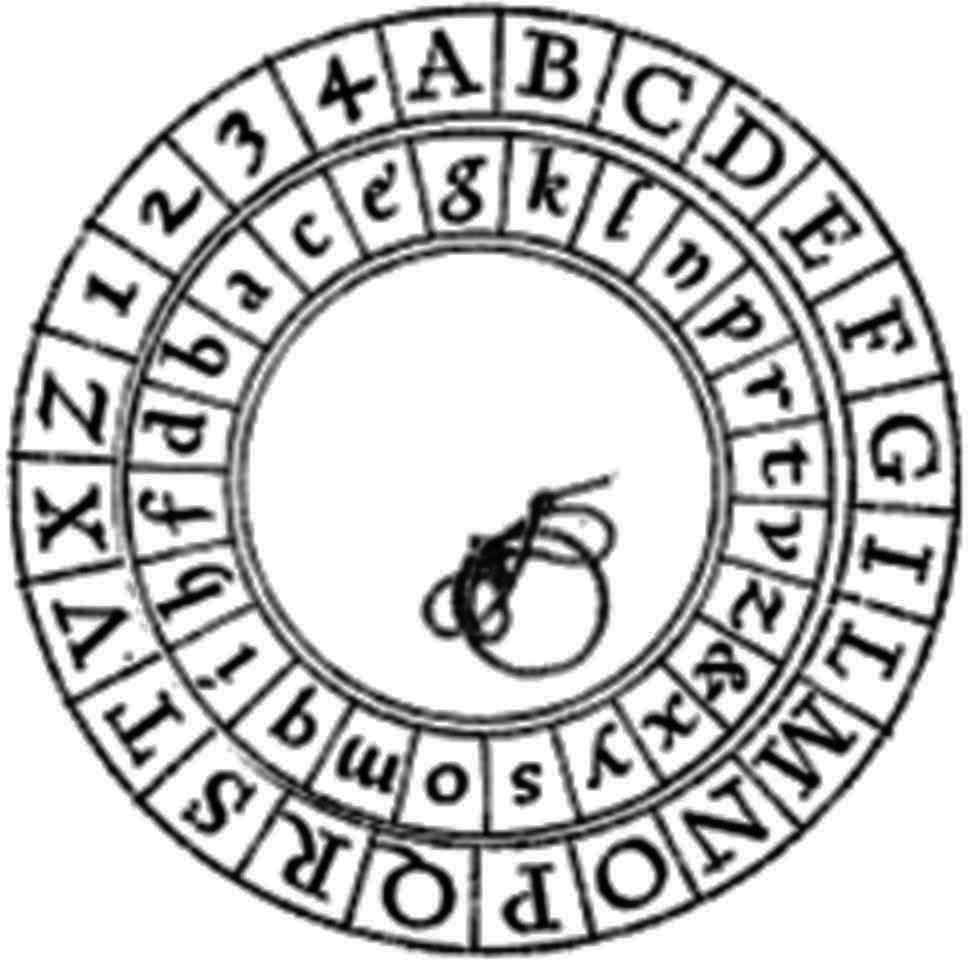
\includegraphics[width=\linewidth]{Alberti_cipher_disk.JPG}
\end{minipage}
\end{frame}

\begin{frame}
\frametitle{Poly-Alphabetic Cipher:\\ Alberti cipher}

\begin{minipage}{0.55\linewidth}
\textbf{Stationary disk}\\
ABCDEFGILMNOPQRSTVXZ1234\\
\textbf{Movable disk}\\
gklnprtuz\&xysomqihfdbace\\

\textbf{Plaintext:}\\
\hspace{4ex}\_LAGVERRA\_...

\textbf{Ciphertext with index g:}\\
\hspace{4ex}AzgthpmmgQ...
\end{minipage}%
\begin{minipage}{0.45\linewidth}
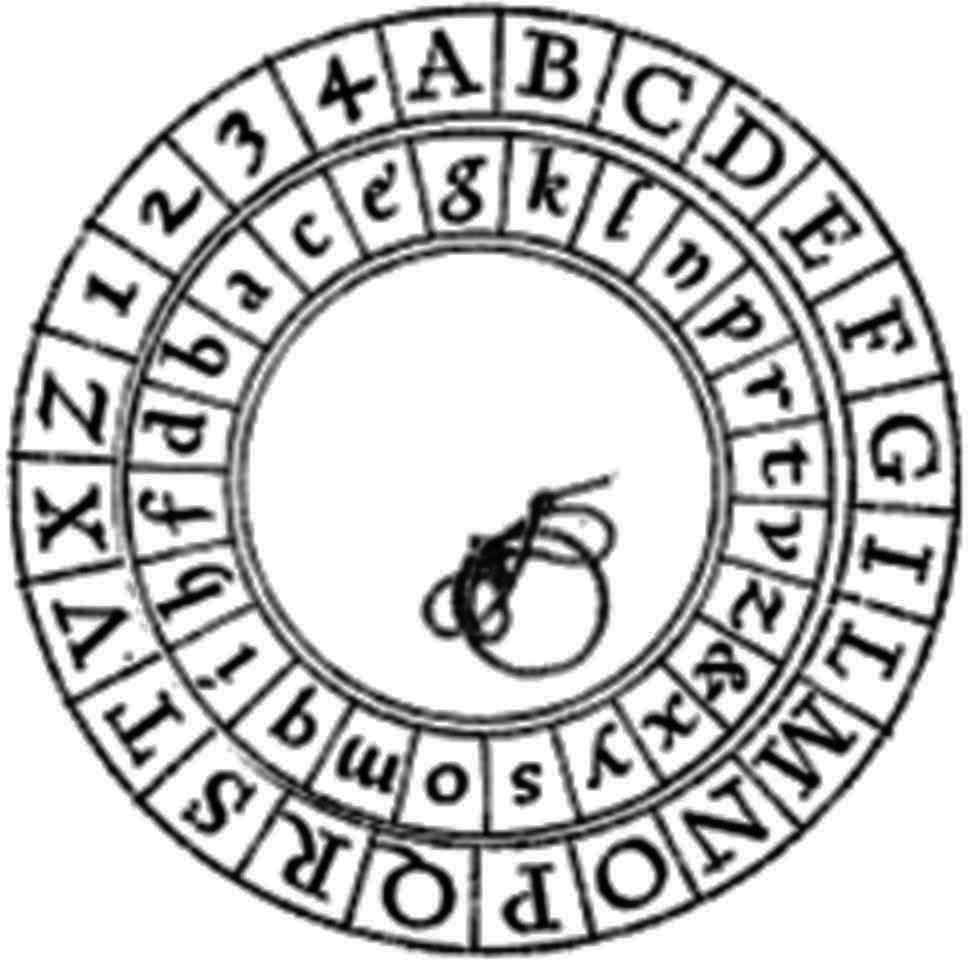
\includegraphics[width=\linewidth]{Alberti_cipher_disk.JPG}
\end{minipage}
\end{frame}

\begin{frame}
\frametitle{Poly-Alphabetic Cipher:\\ VIGENÈRE CIPHER}
\begin{minipage}{0.55\linewidth}
\textbf{Invented by:}\\
Giovan Bellaso $\sim 1553$

\textbf{Works by:}
\begin{itemize}
\item Using a key with a polyalphabetic cipher.
\item Switching alphabet with the key every character.
\item Keep repeating the key over the plaintext.
\end{itemize}
\end{minipage}%
\begin{minipage}{0.45\linewidth}
\centering
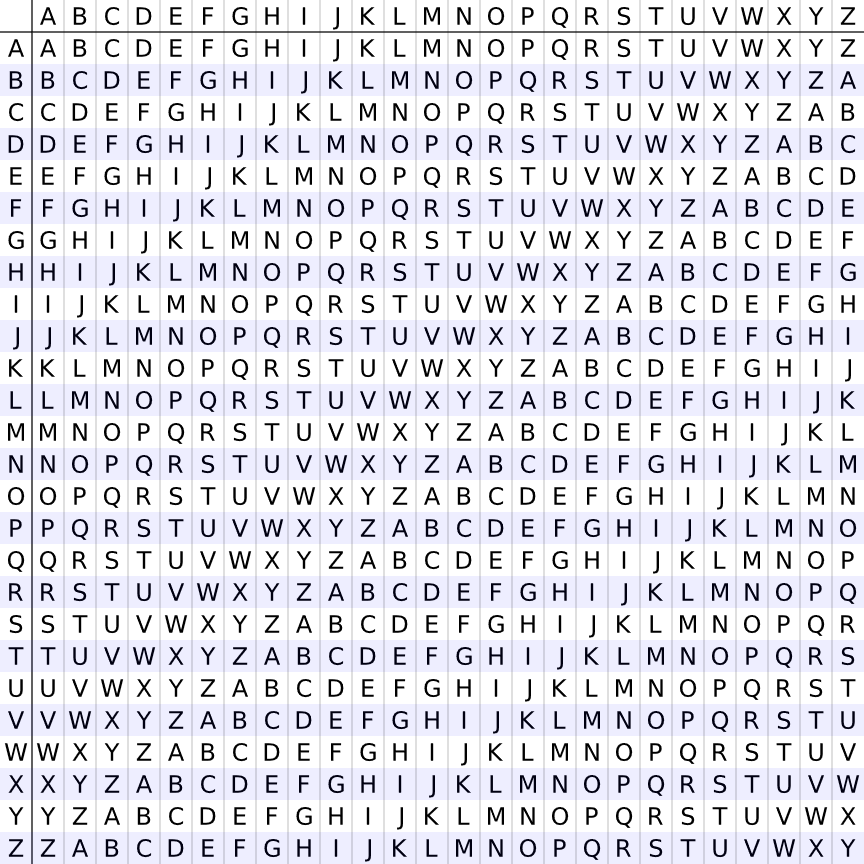
\includegraphics[width=0.95\linewidth]{Vigenere_square_shading} %TABULA RECTA
\end{minipage}
\end{frame}

\begin{frame}
\frametitle{Poly-Alphabetic Cipher:\\ VIGENÈRE CIPHER}
\begin{minipage}{0.55\linewidth}

\textbf{Plaintext:}\\
\hspace{4ex}THEWARSTARTS...

\textbf{KEY=BANANA:}\\
\hspace{4ex}BANANABANANA...

\textbf{Ciphertext:}\\
\hspace{4ex}UHRWNRTTNRGS... 

\end{minipage}%
\begin{minipage}{0.45\linewidth}
\centering
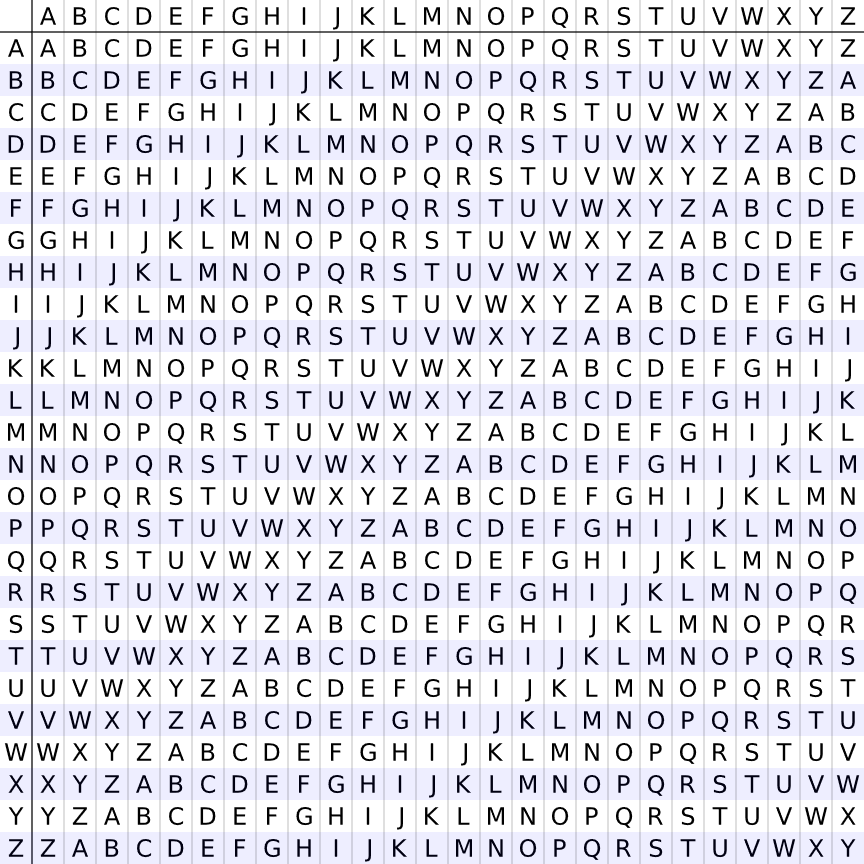
\includegraphics[width=0.95\linewidth]{Vigenere_square_shading} %TABULA RECTA
\end{minipage}
\end{frame}

\subsection{Periodic Polyalphabetic Cipher}
\frame{\tableofcontents[currentsubsection]}

\begin{frame}
\frametitle{Periodic Polyalphabetic Cipher:}
\textbf{Properties:}\\
\hspace{4ex}The frequency distribution is completely flat\\

\textbf{Decoding:}\\
\hspace{4ex}Search for repeating patterns in the ciphertext\\
\hspace{4ex}Get the distance between these patterns, and calculate\\
\hspace{4ex}the greatest common divisor.
\end{frame}

\begin{frame}
\frametitle{Periodic Polyalphabetic Cipher:\\ Problem}
\vspace{-30pt}
\lstinputlisting[
    backgroundcolor=\color{lightgray},
    breakindent=0.5pt,
    breaklines,
    basicstyle={\fontsize{3.2pt}{3.7pt}\selectfont},
    caption=Periodic Poly-Alphabetic Cipher(like Enigma) provided by Mathias,
]{ciphers/polyalphabetic_cipher.txt}
\end{frame}

\begin{frame}
\frametitle{Periodic Polyalphabetic Cipher:\\ Problem}
\begin{minipage}{\linewidth}
\centering
{\fontsize{3.5pt}{4.5pt}\selectfont
\begin{tabular}{ll}\toprule
Character & Frequency in \%     \\
\midrule
F & 6.627456605938891  \\
L & 6.039305695022235  \\
I & 5.666331946636063  \\
Z & 5.035145603213312  \\
E & 4.705207287333238  \\
R & 4.67651699899584   \\
T & 4.045330655573089  \\
' & 3.959259790560895  \\
C & 3.9162243580547984 \\
X & 3.815808348873906  \\
G & 3.686702051355616  \\
J & 3.6723569071869173 \\
; & 3.6723569071869173 \\
P & 3.069860852101564  \\
A & 2.8116482570649834 \\
D & 2.7973031128962846 \\
- & 2.7973031128962846 \\
U & 2.739922536221489  \\
H & 2.5534356620284036 \\
V & 2.4817099411849086 \\
. & 2.438674508678812  \\
S & 2.409984220341414  \\
K & 2.3669487878353177 \\
, & 2.323913355329221  \\
B & 2.194807057810931  \\
Y & 1.6783818677377709 \\
N & 1.6210012910629752 \\
Q & 1.5779658585568785 \\
  & 1.4058241285324917 \\
W & 1.3771338401950939 \\
M & 0.9898149476402237 \\
O & 0.8463635059532348 \\ \bottomrule
\end{tabular}}
\end{minipage}%
\end{frame}

\begin{frame}[containsverbatim]
\frametitle{Periodic Polyalphabetic Cipher:\\ Solution}
\begin{lstlisting}
    qbry = []
    skol = []
    for i in range(0, len(cipher)):
        if(cipher[i:i + 4] == 'QBRY'):
            qbry.append(i)
        elif(cipher[i:i + 4] == 'SKOL'):
            skol.append(i)
    print(qbry)
    print(skol)

    [0, 585, 5550]
    [45, 1060, 1790, 2155, 2250, 3295, 3760, 4490, 4940, 6010]
\end{lstlisting}
\end{frame}

\begin{frame}[containsverbatim]
\frametitle{Periodic Polyalphabetic Cipher:\\ Solution}

\begin{minipage}{0.2\linewidth}
\centering
{\fontsize{3.5pt}{4.5pt}\selectfont
\begin{tabular}{ll}\toprule
Character & Frequency in \%     \\
\midrule
F & 16.91 \\
U & 9.318 \\
Z & 7.383 \\
R & 6.810 \\
S & 5.878 \\
H & 5.806 \\
C & 5.734 \\
D & 5.591 \\
X & 5.017 \\
G & 4.946 \\
; & 3.655 \\
, & 2.795 \\
I & 2.652 \\
P & 2.365 \\
M & 2.150 \\
V & 1.863 \\
Q & 1.792 \\
O & 1.648 \\
. & 1.505 \\
A & 1.505 \\
  & 1.362 \\
Y & 1.003 \\
L & 0.860 \\
W & 0.501 \\
T & 0.215 \\
B & 0.215 \\
N & 0.143 \\
' & 0.143 \\
- & 0.071 \\
K & 0.071 \\
J & 0.071 \\ \bottomrule
\end{tabular}}
\end{minipage}%
\begin{minipage}{0.2\linewidth}
\centering
{\fontsize{3.5pt}{4.5pt}\selectfont
\begin{tabular}{ll}\toprule
Character & Frequency in \%     \\
\midrule
E & 18.72 \\
A & 9.253 \\
T & 7.819 \\
B & 6.671 \\
K & 6.384 \\
X & 5.523 \\
N & 5.236 \\
V & 5.021 \\
. & 4.878 \\
G & 4.878 \\
; & 3.730 \\
R & 3.228 \\
S & 2.654 \\
D & 2.008 \\
J & 1.936 \\
F & 1.793 \\
U & 1.721 \\
L & 1.578 \\
W & 1.506 \\
H & 1.291 \\
C & 1.147 \\
' & 1.147 \\
Y & 0.573 \\
Q & 0.573 \\
I & 0.215 \\
M & 0.215 \\
  & 0.143 \\
- & 0.071 \\
, & 0.071 \\
  &       \\ 
  &       \\ \bottomrule
\end{tabular}}
\end{minipage}%
\begin{minipage}{0.2\linewidth}
\centering
{\fontsize{3.5pt}{4.5pt}\selectfont
\begin{tabular}{ll}\toprule
Character & Frequency in \%     \\
\midrule
J & 15.13 \\
F & 9.397 \\
Z & 7.604 \\
R & 7.317 \\
C & 7.173 \\
I & 6.097 \\
; & 5.380 \\
L & 5.236 \\
' & 5.021 \\
- & 4.304 \\
K & 4.088 \\
Q & 2.725 \\
E & 2.654 \\
, & 2.367 \\
O & 2.008 \\
G & 2.008 \\
H & 1.865 \\
S & 1.578 \\
V & 1.578 \\
M & 1.219 \\
Y & 1.219 \\
U & 1.004 \\
N & 0.932 \\
T & 0.860 \\
  & 0.286 \\
W & 0.286 \\
P & 0.215 \\
B & 0.143 \\
. & 0.143 \\
D & 0.071 \\
A & 0.071 \\ \bottomrule
\end{tabular}}
\end{minipage}%
\begin{minipage}{0.2\linewidth}
\centering
{\fontsize{3.5pt}{4.5pt}\selectfont
\begin{tabular}{ll}\toprule
Character & Frequency in \%     \\
\midrule
L & 18.00 \\
P & 10.32 \\
T & 6.456 \\
, & 6.384 \\
D & 6.312 \\
' & 5.882 \\
Y & 5.523 \\
. & 5.523 \\
F & 4.949 \\
Z & 4.734 \\
B & 3.515 \\
X & 2.797 \\
I & 2.654 \\
H & 2.439 \\
W & 2.439 \\
R & 2.152 \\
V & 1.793 \\
N & 1.721 \\
A & 1.578 \\
  & 1.362 \\
Q & 0.789 \\
K & 0.645 \\
J & 0.573 \\
O & 0.502 \\
E & 0.430 \\
S & 0.215 \\
U & 0.143 \\
M & 0.071 \\
G & 0.071 \\
  &       \\ 
  &       \\ \bottomrule
\end{tabular}}
\end{minipage}%
\begin{minipage}{0.2\linewidth}
\centering
{\fontsize{3.5pt}{4.5pt}\selectfont
\begin{tabular}{ll}\toprule
Character & Frequency in \%     \\
\midrule
I & 16.71 \\
- & 9.540 \\
' & 7.604 \\
G & 6.527 \\
X & 5.738 \\
; & 5.595 \\
C & 5.523 \\
Z & 5.451 \\
T & 4.878 \\
L & 4.519 \\
R & 3.873 \\
  & 3.873 \\
P & 2.439 \\
V & 2.152 \\
W & 2.152 \\
Q & 2.008 \\
S & 1.721 \\
E & 1.721 \\
A & 1.649 \\
U & 1.506 \\
H & 1.362 \\
M & 1.291 \\
J & 0.645 \\
K & 0.645 \\
B & 0.430 \\
. & 0.143 \\
O & 0.071 \\
F & 0.071 \\
Y & 0.071 \\
N & 0.071 \\
  &       \\ \bottomrule
\end{tabular}}
\end{minipage}%
\end{frame}

\begin{frame}[containsverbatim]
\frametitle{Periodic Polyalphabetic Cipher:\\ Solution}
\vspace{-20pt}
\begin{lstlisting}[
    backgroundcolor=\color{lightgray},
    breakindent=0.5pt,
    breaklines,
    basicstyle={\fontsize{3.2pt}{3.7pt}\selectfont},
    caption=Periodic Poly-Alphabetic Cipher(like Enigma) provided by Mathias,
]
within henry's mind the expedient of dispatching the  oung knight as bearer of his own death warrant had been conceived in a spirit of absurd bravado. so far as his calculating and selfish character permitted, he was fond of him. but if he suffered a regret, it was who ly personal, and because of circumstances that had compelled him to part from one in whose companionship he had derived a great deal of pleasure. in respect of any feeling of genuine sorrow, the entire scene enacted between himse f and stanley had been a comp ete farce. though he had invested that doughty warrior with man  and distinguished honors and great power, he had never entertained on the behalf of his chief official that feeling of confidence so essential to the comp aisance of mind of any ruler. it was his intention to set before that individua  an examp e of integrit  and devotion that the king fancied would be well worthy of emulation. as an additional safeguard, however, he caused secret spies of his own selection to be dispatched in the train of sir richard. in adopting this course he believed himself to be keeping the situation well in hand; at once guarding against any interruption of the final delivery of the unusual warrant, and providing him with the means of testing lord stan ey's devotion to his cause. thus, had not sir richard taken it into his head to follow an itinerar  entirely different from either the one suggested by henry, or that secretly transmitted to him beside the portcullis b  lord stan ey, some state prob ems of vast magniture and importance might then have been solved. as it subsequentl  transpired, al  along and between the roads that it was definite y supposed the young knight and his squire would make their pilgrimage, king's emissaries were constantly meeting and receiving entertainment of stan ey's lieutenants, as wel  as the other way about. obviousl , neither the one side nor the other dared to hint of its purpose of espionage or destination; nor  et dared to display any undue haste in parting to pursue its secret way. it also became necessary for them to observe every possib e precaution in the matter of covering up their trails, one from another; and, in this way, the innocent cause of this rather amusing game of cross-purposes was permitted to go unmolested upon his way. the route that sir richard had chosen rendered it necessary for himself and squire to tread paths and by-ways used chiefl  by peasant farmers and sheep-herders. at times, after a heavy fa l of rain, such of these as wound through the low lying val eys would become wholly impassable, making it needful for our pi grims to await the draining of the flood into the rivers, or to make  ong detours to come upon the other side. for this reason, it had reached well a ong into october before they had passed through the liberties of berwick and set foot upon scottish soil. it was growing late in the afternoon of their second day in scotland, and while they were skirting the edge of a rock-tarn  ying in g oom  seclusion in the middle of a desolate moor, that sir richard was murderous y deprived of the services of his squire and brave attendant. there had been no hint of the approach of the tragedy; no clue as to the identity or purpose of the cowardly perpetrators following its occurrence. mounted upon his mettlesome charger, which, though uncommon y powerfu , was somewhat fatigued because of the many miles put behind him that day, the young knight was riding s owl  along some two hundred  ards in advance of belwiggar. the sky was heavy, gray, and lowering; and the bou der-strewn, monotonousl  leve  expanse of moor affording no pleasant aspect or interesting contrasts to the eye, sir richard's gaze remained fixed upon the nodding head of his sta lion. so near the brink was the narrow path winding along the waters of the tarn, and so unruffled was its surface, that steed and armored rider were mirrored faithfull , point for point, beneath. hearing a sharp rattling of stee -shod hoofs behind him, and vaguely marveling as to the cause of this unexpected and unusual burst of energy upon the part of his squire, the young knight turned, with a smile upon his face, to greet belwiggar's approach. to his horrified surprise he was but just in time to see the honest fellow writhing in an agony of death, while the horse that he had so  ately bestrode in the prime vigor of rugged health whisked blind y ahead of the young knight a ong the road, till, crashing against a huge boulder upreared within its path, it stumbled, seemed to hang for an instant in mid-air, and then, neighing with wi d affright, disappeared with a tremendous sp ash beneath the surface of the tarn. apprehending some immediate danger to himself, sir richard, upon the instant, drew his visor close. just as he had accomplished this move a bo t struck fair upon the joint of his neck-guard; and, though it did him no harm beyond causing his head to ring with the force of the impact, it was the cunning of his armorer alone that had saved him from a death similar to that of be wiggar. having no means of knowing the exact direction from whence the arrows had been sped, and the nature of the ground precluding the possibi ity of sending his horse over it, the  oung knight made no attempt to seek out and punish his assai ant. he shot a glance of the keenest scrutiny from bou der to boulder, but there was no sign of a living being upon the moor. satisfied that belwiggar's death must go unavenged for the time, he rode back to where he la  with a feathered shaft, still quivering, protruding from his broad breast. he dismounted beside the bod , tethering his horse in the hollow between two rocky promontories through which the path swung. he stood looking around him for a space, uncertain what to do. so overwhe ming y appalling and strange were the circumstances attending the tragedy, and to that degree was sir richard oppressed by his me ancholy surroundings, that he became fi led with a fee ing of unspeakable dread, an almost uncontro lable desire to throw himself upon the back of his steed and gal op swiftly away. torn b  such emotions, it was no light task to remain upon the scene for the purpose of making such disposition of poor be wiggar's body as his limited means would permit. by employing the dead warrior's battle-ax in  ieu of mattock, however, he contrived to hol ow out a sufficient space to  ay him decently away. then, piling up a mound of  oose stones above the shallow grave, sir richard remounted and pursued his solitary way northward toward bannockburn and castle  ewe. as he journeyed onward the young knight made many determined efforts to whistle and sing away a feeling of deep melancho y that persisted in setting somber y down upon him. in the manner of a gloomy procession passing in review before his mind's eye, he recalled al  of the wild folklore with which his ears had been beguiled since his advent into scotland
\end{lstlisting}
\end{frame}

\subsection{Running Key Cipher}
\frame{\tableofcontents[currentsubsection]}

\begin{frame}
\frametitle{Running Key Cipher:\\ Example}

\textbf{Plaintext:}\\
f   l   e   e   a   t   o   n   c   e   w   e   a   r   e   d   i   s   c   o   v   e   r   e   d\\
\textbf{Running key:}\\
E   R   R   O   R   S   C   A   N   O   C   C   U   R   I   N   S   E   V   E   R   A   L   P   L\\
\textbf{Ciphertext:}\\
J   C   V   S   R   L   Q   N   P   S   Y   G   U   I   M   Q   A   W   X   S   M   E   C   T   O\\
\end{frame}

\begin{frame}
\frametitle{Running Key Cipher:\\ Problem}
\vspace{-30pt}
\lstinputlisting[
    backgroundcolor=\color{lightgray},
    breakindent=0.5pt,
    breaklines,
    basicstyle={\fontsize{2.6pt}{2.9pt}\selectfont},
    caption=Running Key Cipher provided by Mathias,
]{ciphers/running_key_cipher.txt}
\end{frame}

%------------------------------------------------
%################################################
\section{Modern Ciphers}
\frame{\tableofcontents[currentsection]}
%------------------------------------------------
\begin{frame}
\frametitle{Modern Ciphers}

\begin{itemize}
    \item Private-key cryptography, where the same key is used for encryption
        and decryption.
    \item Public-key cryptography, where two different keys are used for
        encryption and decryption.
\end{itemize}
Ciphers can be distinguished into two types by the type of input data:
\begin{itemize}
    \item Block ciphers, which encrypt block of data of fixed size
    \item Stream ciphers, which encrypt continuous streams of data
\end{itemize}
\end{frame}

\begin{frame}
\frametitle{AES}
\includegraphics[width=\linewidth]{aes}
\end{frame}
%################################################
%------------------------------------------------
\section{End}
%------------------------------------------------
\begin{frame}
\frametitle{Conclusion}
\Large{\centerline{Conclusion}}
\end{frame}

\begin{frame}
\Large{\centerline{Questions?}}
\end{frame}
%------------------------------------------------
%################################################
\end{document}